% Comment this line out if you need a4paper
%\documentclass[letterpaper, 10 pt, conference]{ieeeconf}  
% Use this line for a4 paper
\documentclass[a4paper, 10pt, conference]{ieeeconf}
\IEEEoverridecommandlockouts                              
\overrideIEEEmargins                                      
% Needed to meet printer requirements.
% See the \addtolength command later in the file to balance the column lengths on the last page of the document
\usepackage{cite}
\usepackage{amsmath,amssymb,amsfonts}
\usepackage{algorithmic}
\usepackage{graphicx}
\usepackage{textcomp}
\def\BibTeX{{\rm B\kern-.05em{\sc i\kern-.025em b}\kern-.08em
    T\kern-.1667em\lower.7ex\hbox{E}\kern-.125emX}}
    
\title{\LARGE \bf
Non-zero Setpoint Tracking for a Dual-Axis Tilting Quadrotor Helicopter
}
\author{Nicholas Von Klemperer$^{1}$ and Edward Boje$^{2}$% <-this % stops a space
\thanks{$^{1}$MSc (Eng) Candidate, Engineering \& the Built Environment, Faculty of Electrical Engineering, University of Cape Town, Cape Town, South Africa
{\tt\small nicholas.vonklemperer@alumni.uct.ac.za}}
\thanks{$^{2}$Professor and Head of department, Faculty of Electrical Engineering, University of Cape Town, Cape Town, South Africa,
        {\tt\small edward.boje@uct.ac.za}}%
}
\begin{document}



\maketitle
\thispagestyle{empty}
\pagestyle{empty}
%=========================================================
\begin{abstract}
%=========================================================
This work applies non-zero attitude and position setpoint tracking to a quadrotor helicopter; achieved by mechanically solving the problem of a quadrotor's inherent underactuation. Introduction of overactuation results in a multibody, non-linear system to be modelled and stabilized. High level setpoint tracking controllers design virtual control inputs which are then allotted out to the plant's actuators by a lower level allocation rule. The non-linear state-space controller(s) are optimized iteratively using a swarm algorithm; producing a control suite that successfully tracks an orbital trajectory.
%=========================================================
\end{abstract}
%=========================================================
\textbf{\emph{Index terms}--- control, non-linear, over actuated, optimization, quadrotor}
%=========================================================
\section{INTRODUCTION}
%=========================================================
Quadrotor helicopters, first puplished in \cite{x4flyer}, are currently an extremely popular field of control research. As almost every quadrotor based papers will mention; this is due to a recent advent in cheap embedded systems for implementation of the UAV's control loop. Quadrotor helicopters are inherently underactuated, making the control plant ill-posed. Their control problem is design of 4 controllable inputs (namely the four propeller's rotational speed) to articulate a 6 degree of freedom (\emph{DOF}) body. Standard control solutions linearize the plant around the attitude's origin; reducing the degrees of controllable freedom the system has. What follows is a proposal that achieves non-zero setpoint tracking for a quadrotor by introducing overactuation to the vehicle, apply no such linearisation to the dynamic equations of motion. A high level control law designs net torque and force inputs to be applied to the multibody vehicle about it's center of motion. A lower level allocation rule then allots out that virtual control input amongst the actuator set to be physically implemented.
\par
Over actuated control is most common in the context of satellite attitude control. Typically a satellite's extra actuators are included for the sake of fault tolerance, implemented only when higher priority acutators fail mechanically. Fault tolerant control for satellites is discussed in \cite{ftcallocation}, where the additional actuators are included for redundancy rather than complementing a control input. Alternatively, \cite{quaternionbackstep} implemented quaternion based backstepping to track a satellite's orbital trajectory whilst making use of all available actuators, using a pseudo-inversion allocation rule. 
\\
A series of allocation schemes is surveyed in \cite{allocation}, most allocation applies some sort of inversion to find explicit actuator positions.
\par
Not much work has been done on reconfigurable aerospace vehicles. The only commerical example is the DJI Inspire1 which only can raise or lower it's support arms. Reconfigurable aerospace frames are usually avoided due to their dynamic complexities. Dual-axis tilting capabilities are often incorporated into birotor aircraft; \cite{ggress} presented a dual-axis tilting bi-rotor design but in the control constrained the actuation to an effective single axis of tilt. In the case of tilting quadrotor aircraft, \cite{tiltingmodelling} proposed a single co-axial rotation of a quadrotor's propellers which was subsequently tested in \cite{tiltingtest}. Another paper, \cite{nemati}, similarly proposed a single axis tilting quadrotor aircraft. Neither single axis quadrotor papers consider the dynamic consequences of reconfiguring the quadcopter mid-flight. The only dual-axis tilting quadrotor work, \cite{tiltgasco}, treats the control inputs as a regular fixed axis quadrotor, but with an introduced actuator plant that produces gyroscopic torque from pitching/rolling the rotating propeller module.
\par
The remainder of this paper is arranged as follows; the prototype's design and it's reference conventions are briefly described in \ref{sec:design}. Thereafter, \ref{sec:dynamics} presents the state differential dynamic model used for 6-DOF equations of motion, including the multibody non-linearities which stem from the prototype's structure and mid-flight reconfiguration. Position and attitude controllers are derived in \ref{sec:control}, together with an allocation rule. Each control law's coefficients are designed using a swarm optimization discussed in \ref{sec:optimization}. Finally setpoint tracking is empirically tested in \ref{sec:setpoint} with conclusions drawn in \ref{sec:conclusion}.
%=========================================================
\section{Design and Conventions} 
\label{sec:design}
%=========================================================
Two Cartesian reference frames are considered here; first the fixed inertial frame $\mathcal{F}^{I}$ which all motion is taken with respect to. Secondly the body frame $\mathcal{F}^{b}$ which is attached and centred on the vehicle itself. Rotation (or \emph{transformation}) of some vector $\vec{v}_I$ from the inertial frame to the body frame is applied by a quaternion operation:
\begin{equation}\label{eq:quaternion-operation}
v_b=Q_b\otimes \vec{v}_I \otimes Q_b^*~~~~\in\mathcal{F}^{b}
\end{equation}
Wherein $Q_b=\begin{bmatrix}q_0 & \vec{q}\hspace{2pt}\end{bmatrix}^T$ is the attitude's quaternion, $Q_b^*$ is the quaternion complex conjugate and $\otimes$ is the hamilton product between two quaternions. Quaternions are detailed thoroughly in \cite{shoemaker}, if such concepts are unfamiliar to the 
reader\ldots
\par
\begin{figure}[tbp]
\centering
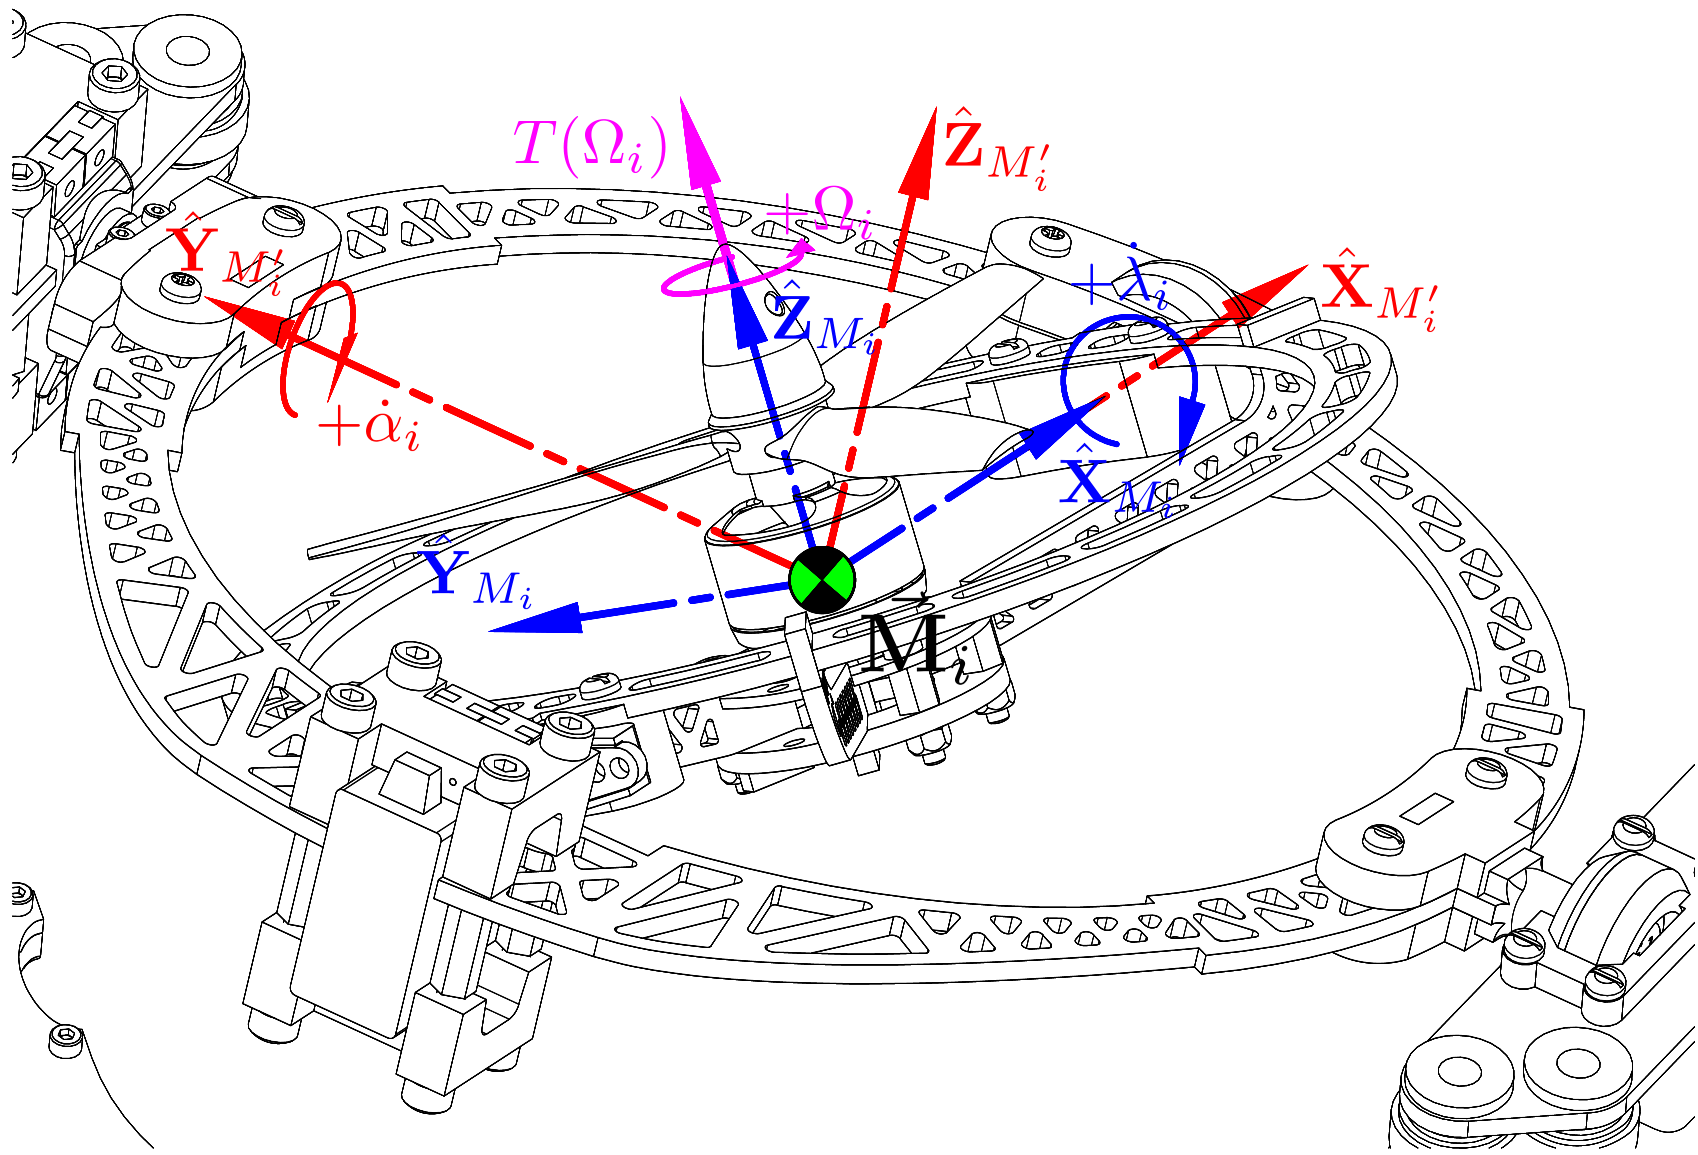
\includegraphics[width=0.5\textwidth]{figs/force-redirect}
\vspace{-20pt}
\caption{Actuator motor module}
\label{fig:force-redirect}
\vspace{-16pt}
\end{figure}
\par
The prototype extends the actuation suite of a regular quadcopter, such as \cite{x4flyer}, to an overactuated 12-\emph{DOF} system by introducing 8 additional actuator plants. A standard quadrotor consists of only 4 controllable inputs; namely each of the propeller's rotational speeds $\Omega_{1\rightarrow 4}$, under actuating the control plant. The design here adds 2 revolute actuators to respectively pitch and roll \emph{each} of the 4 motors and propellers about their $\hat{X}_{M_i}$ and $\hat{Y}_{M_i}$ axes, aligned as per Fig:\ref{fig:force-redirect}.
\par
The \emph{motor module} frame $\mathcal{F}^{M_i}$ is attached to the $i^{\text{th}}$ motor ($i\in[1:4]$), whose propeller produces an input thrust in the $\hat{Z}_{M_i}$ axis direction of it's frame. The two actautors rotate the motor/propeller in sequential gimbal-like fashion; first about it's $\hat{X}_{M_i}$ axis by an angle of $\lambda_i$. Then about an intermediate frame's $\hat{Y}_{M_i'}$ axis by an angle of $\alpha_i$. The resultant thrust vector $\vec{T}(\Omega_i)$ in the $\hat{Z}_{M_i}$ direction is calculated using blade-element-momentumn (\emph{BEM}) theory, \cite{nonlineardynamics}. Thrust and power coefficients, $C_T$ and $C_P$ respectively, relate the propeller's rotational speed in $[\text{RPS}]$ to it's produced thrust and aerodynamic torque as per:
\begin{subequations}\label{eq:bem}
\begin{equation}\label{eq:bem-thrust}
\vec{T}(\Omega_i)=C_T(J)\rho\Omega_i^2D^4\cdot\hat{Z}_{M_i}~~~~[\text{N}]
\end{equation}
\vspace{-12pt}
\begin{equation}\label{eq:bem-torque}
\vec{\tau}_Q(\Omega)_i=C_P(J)\rho\Omega_i^3D^5(1/R\Omega_i)\cdot\hat{Z}_{M_i}~~~~[\text{Nm}]
\end{equation}
\end{subequations}
Where $J$ is the propeller's advance ratio, $\rho$ is the air density taken  at \emph{STP} and $D$ is the propeller's diameter in $[\text{m}]$. Further details of BEM theorey and a propeller's aerodynamics are presented in \cite{nonlineardynamics}. Each thrust and power coefficient used was linearly interpolated from data in \cite{lowreynolds} to match physical tests applied to the hardware under consideration.
\par
Each of the four motor modules, in Fig:\ref{fig:force-redirect}, are aligned relative to the body frame's center $\vec{\mathbf{O}}_b$ as per Fig:\ref{fig:body-frame}. The $1^{\text{st}}$ and $3^{\text{rd}}$ motor modules have their positive and negative $\pm\hat{X}_{M_1/M_3}$ axes aligned with the body frame's $\hat{X}_b$ axis. While the $2^{\text{nd}}$ and $4^{\text{th}}$ modules have their positive and negative $\pm\hat{Y}_{M_2/M_4}$ axes aligned with the $\hat{Y}_b$ body frame's axis. Motors $1$ and $3$ have clockwise propeller rotations, $+\Omega_{1/3}$, whereas motors $2$ and $4$ have anti-clockwise propeller rotations, $-\Omega_{2/4}$. An instantaneous configuration of the multibody system is fully described by the 4 propeller's rotational speed and the 8 additional actuator rotational positions. 
\par
That actuator configuration input matrix $u$, within the saturation limited actuator subset $\mathbb{U}$, is such that:
\begin{equation}\label{eq:actautor-matrix}
\underset{\in\mathbb{U}}{u}\triangleq\begin{bmatrix}
\Omega_1 & \lambda_1 & \alpha_1 & \ldots & -\Omega_4 & \lambda_4 & \alpha_4
\end{bmatrix}^T~~\in\mathbb{R}^{12}
\end{equation}
A propeller's generated thrust or torque, (\ref{eq:bem-thrust}) and (\ref{eq:bem-torque}) respectively, has the body frame vector counterpart:
\begin{subequations}
\begin{equation}\label{eq:force-redirect}
\vec{T}_{1\rightarrow 4} = Q_{M_i}^*\otimes\vec{T}(\Omega_i)\otimes Q_{M_i}~~[\text{N}],~\in\mathcal{F}^{b}
\end{equation}
\vspace{-16pt}
\begin{equation}\label{eq:torque-redirect}
\vec{Q}_{1\rightarrow 4} = Q_{M_i}^*\otimes\vec{Q}(\Omega_i)\otimes Q_{M_i}~~[\text{Nm}],~\in\mathcal{F}^{b}
\end{equation}
Where each $Q_{M_i}$ is the relative quaternion from the motor module's frame $\mathcal{F}^{M_i}$ to the body frame $\mathcal{F}^{b}$ such that:
\begin{equation}
Q_{M_i}\triangleq Q_z(\sigma_i)\otimes Q_y(\alpha_i) \otimes Q_x(\lambda_i)
\end{equation}
\end{subequations}
With $Q_z,Q_y$ and $Q_x$ being quaternion rotations about each $\hat{Z},\hat{Y}$ and $\hat{X}$ axes respectively. Note that $\sigma_i$ is the $\hat{Z}_b$ orthogonal angular rotation between each motor module; detailed in the layout of Fig:\ref{fig:body-frame}. The net heave and control torque acting on the body due to actuation action is simply:
\begin{subequations}\label{eq:net-inputs}
\begin{equation}\label{eq:net-force}
\vec{F}_{\mu}=\sum_{i=1}^{4}\vec{T}(\Omega_i,\lambda_i,\alpha_i)~~~~[\text{N}]
\end{equation}\vspace{-10pt}
\begin{equation}\label{eq:net-torque}
\vec{\tau}_{\mu}=\sum_{i=1}^4\vec{L}_{i}\times\vec{T}(\Omega_i,\lambda_i,\alpha_i)+\vec{\tau}_Q(\Omega_i,\lambda_i,\alpha_i)~~~~[\text{Nm}]
\end{equation}
\end{subequations}
Each thrust vector $\vec{T}(\Omega_i,\lambda_i,\alpha_i)\in\mathcal{F}^b$ is a combined function of (\ref{eq:bem-thrust}) and (\ref{eq:force-redirect}). The net torque $\vec{\tau}_\mu\in\mathcal{F}^b$ comprises of differential torque arm cross-products from input thrusts $\vec{T}_{1\rightarrow 4}$ each acting at a length $\vec{L}$ in Fig:\ref{fig:body-frame} \emph{and} the propeller's aerodynamic torque, $\vec{\tau}_Q(\Omega_i,\lambda_i,\alpha_i)$, as a combined function of (\ref{eq:bem-torque}) and (\ref{eq:torque-redirect}). The latter aerodynamic torque $\sum\vec{\tau}_Q(\Omega_i,\lambda_i,\alpha_i)$ is a term to be \emph{compensated} for in feedback, not used as a controllable input.
\par
\begin{figure}[bp]
\vspace{-15pt}
\centering
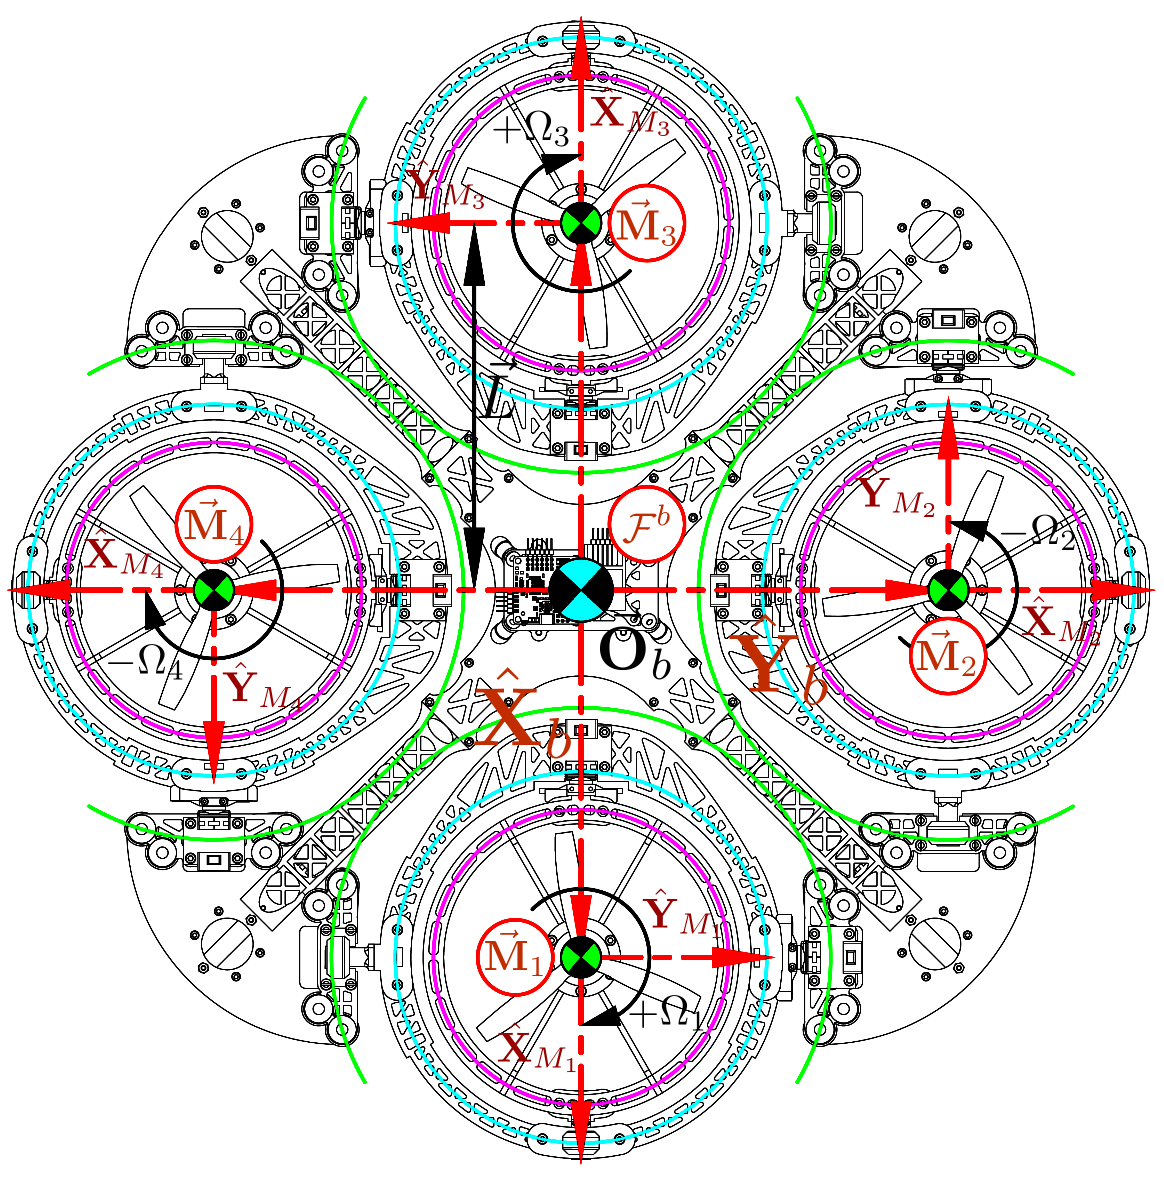
\includegraphics[width=0.5\textwidth]{figs/body-frame}
\vspace{-18pt}
\caption{Body frame axes layout}
\label{fig:body-frame}
%\vspace{-15pt}
\end{figure}
%=========================================================
\section{Dynamics}
\label{sec:dynamics}
%=========================================================
The typical Lagrangian dynamics for a \emph{rigid} 6-DOF body are as follows; derived from first principles in\cite{dualaxistilting}. For a rigid body with an angular velocity $\vec{\omega}_b$ in $\mathcal{F}^b$ and an inertial matrix $J_b$ aligned with axes in $\mathcal{F}^b$; the quaternion dynamics for the attitude's differential equations of motion are:
\begin{subequations}\label{eq:attitude-dynamics}
\begin{equation}\label{eq:quaternion-deriv}
\dot{Q}_b=1/2\big(Q_b\otimes\vec{\omega}_b\big)~~\in\mathcal{F}^I
\end{equation}
\vspace{-16pt}
\begin{equation}\label{eq:attitude-dynamics.b}
\dot{\vec{\omega}}_b= J_b^{-1}\big(-\vec{\omega}_b\times J_b\vec{\omega}_b+\vec{\tau}_\mu\big)~~[\text{rad.s}^{-2}],~\in\mathcal{F}^{b}
\end{equation}
\end{subequations}
For a net torque control input $\vec{\tau}_\mu\in\mathcal{F}^b$. Similarly the vehicle's translational dynamics, for an iniertial position $\vec{\mathcal{E}}\in\mathcal{F}^{I}$ and a translational velocity $\vec{v}_b\in\mathcal{F}^b$ and a net input force $\vec{F}_\mu\in\mathcal{F}^b$:
\begin{subequations}\label{eq:position-dynamics}
\begin{equation}
\dot{\vec{\mathcal{E}}}=Q_b^*\otimes\vec{v}_b\otimes Q_b~~[\text{m.s}^{-1}],~\in\mathcal{F}^{I}
\end{equation}
\vspace{-16pt}
\begin{equation}\label{eq:postion-dynamics.b}
\dot{\vec{v}}_b=m_b^{-1}\big(-\vec{\omega}_b\times\vec{v}_b+m_b\vec{G}_b+\vec{F}_\mu\big)~~[\text{m.s}^{-2}],~\in\mathcal{F}^{b}
\end{equation}
\end{subequations}
For a mass $m_b$ and a gravitational acceleration $\vec{G}_b$ transformed to the body frame. Particulars associated with the multibody dynamics resulting from the system's actuation were additively introduced to the above equations of motion (\ref{eq:attitude-dynamics}) and (\ref{eq:position-dynamics}). Furthermore, explicit calculation of the instantaenous net inertial matrix is not a constant $J_b$ but a function the acutator matrix (\ref{eq:actautor-matrix}); $J_b(u)$. The complete multibody dynamics for the design are presented in \cite{dualaxistilting}, from which this paper is adapted, but are excluded here for the sake of brevity. In summary; each of the 13 independent bodies are revolutely connected with only one permissible degree of rotational freedom between each sequential structure. Fig:\ref{fig:response-body} shows the exploded components of a single motor module; each with their own rotational velocity relative to $\mathcal{F}^b$, resulting from the actuation rates $\dot{\lambda_i}$ and $\dot{\alpha_i}$. The non-Newtonian frames for each rotating sub-body made quantifying the net multi-body's response to rotational and translational motion highly complicated. A complete Lagrangian, \cite{lagrange}, was constructed for each body's net kinetic and potential energies. As per Lagrangian dynamics, the partial derivatives with respect to the Lagrangian's path co-ordinates results in the \emph{generalized forces}, in this case torques $\vec{\tau}_b$, acting on the system. 
\begin{figure}[bp]
\vspace{-15pt}
\centering
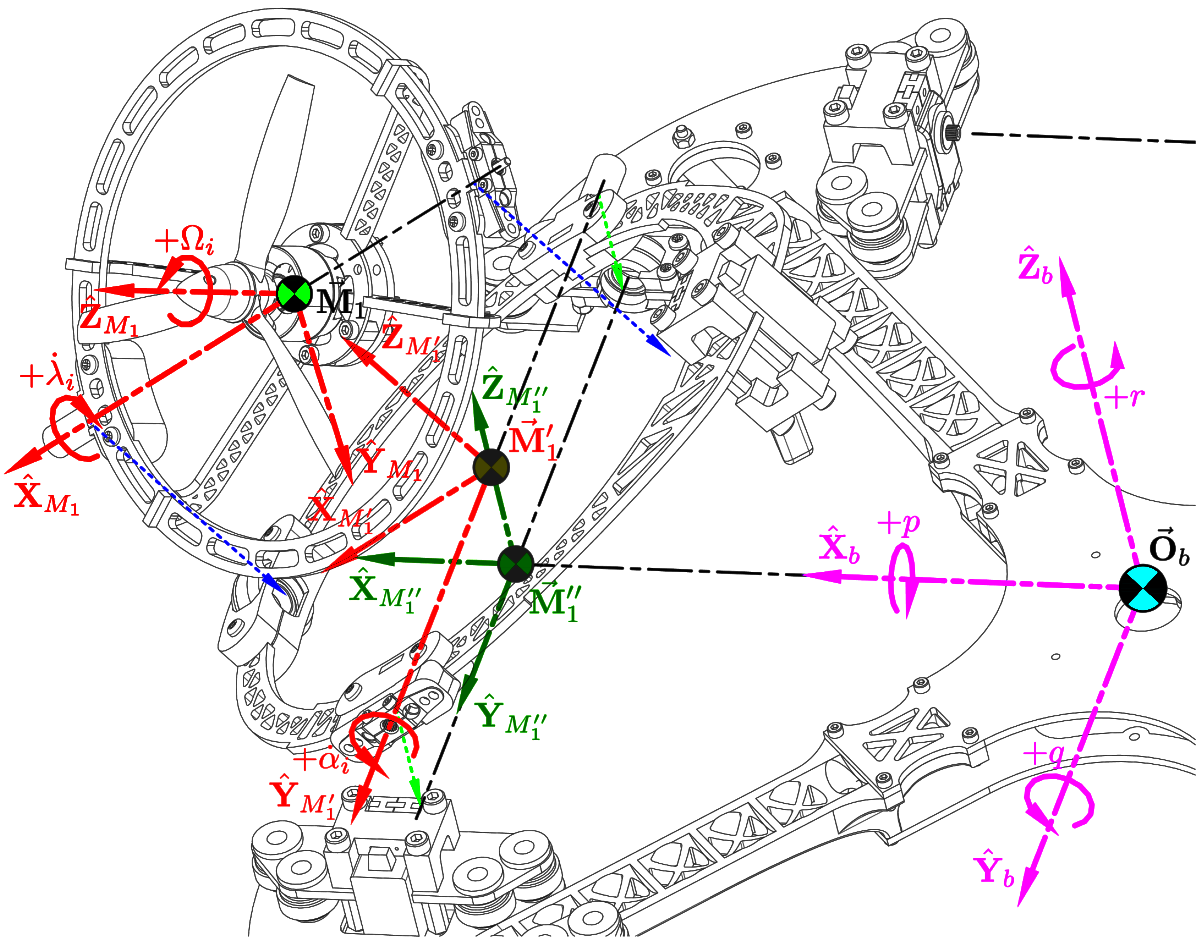
\includegraphics[width=0.5\textwidth]{figs/response-body}
\vspace{-22pt}
\caption{Multi-body overview}
\label{fig:response-body}
\vspace{-3pt}
\end{figure}
\newpage
Each motor module contributes some non-zero inertial derivative towards the dynamic response calculations, complicating their solutions. If a body has an inertia $J$ in it's principle frame, but the body is rotated by $\theta$ about some unit axis $\hat{u}$. The effective transformed inertia is:
\begin{subequations}
\begin{equation}\label{eq:inertia}
J'=R_{\hat{u}}(\theta)\big(J\big)R_{\hat{u}}^{-1}(\theta)
\end{equation}
Where $R_{\hat{u}}(\theta)$ is the rotation matrix about that unit axis, \cite{rotation}. Quaternions are ill suited for inertial transformations; hence the use of rotation matrices here. If $\theta$ is a time varying angular rotation then (\ref{eq:inertia}) has a time derivative 
\begin{equation}
\dot{J}'=d/dt\Big(R_{\hat{u}}(\theta)\big(J\big)R_{\hat{u}}^{-1}\Big)
\end{equation}
\vspace{-18pt}
\begin{multline}\label{eq:inertia-rate}
=[\dot{\vec{\theta}}\hspace{2pt}]_\times R_{\hat{u}}(\theta)\big(J\big)R_{\hat{u}}^{-1}(\theta)+R_{\hat{u}}(\theta)\big(\dot{J}\big)R_{\hat{u}}(\theta)
\\
-R_{\hat{u}}(\theta)\big(J\big)[\dot{\vec{\theta}}\hspace{2pt}]_\times R_{\hat{u}}^{-1}(\theta)
\end{multline}
Where $\vec{\theta}$ is the projected vector of $\theta$ in the direction of it's unit axis $\hat{u}$, or that $\vec{\theta}\triangleq\theta\cdot\hat{u}$. Then $\dot{J}$ is the inertia's time derivative (if any) in it's principle frame. Finally $[.]_{\times}$ is such that a two vector cross product $\vec{a}\times\vec{b}$, is applied as a matrix multiplication:
\begin{equation}
\vec{a}\times\vec{b}\equiv [\vec{a}\hspace{2pt}]_{\times}\vec{b}
\end{equation}
\end{subequations}
A body's \emph{generalized force} (torque) response to an applied angular velocity/acceleration consists of three components; an inertial rate component, an inertial response to the applied acceleration and a gyroscopic cross-product of the relative angular velocities. Those net responses are lumped into an additive toque term $\hat{\tau}_b(u)$ which, like the body's net rotational inertia, is a function of the actuator configuration $u\in\mathbb{U}$. The multibody response derivation is, however, far too cumbersome to include here and so is omitted for conciseness. The angular differential equation, (\ref{eq:attitude-dynamics}), then treats the net aerodynamic torque $\vec{\tau}_Q$ from (\ref{eq:net-torque}) and the multibody non-linearity responses $\hat{\tau}_b(u)$ as terms to be compensated for:
\begin{subequations}
\begin{multline}\label{eq:angular-diff}
\therefore \dot{\vec{\omega}}_b = J_b(u)^{-1}\big(-\vec{\omega}_b\times J_b(u) \vec{\omega}_b-\hat{\tau}_b(u)
\\
+\vec{\tau}_Q+\vec{\tau}_g+\vec{\tau}_\mu \big)
\end{multline}
Lastly, the torque $\vec{\tau}_g$ is from the eccentric center of gravity produced by rotated motor modules. The net center of gravity is $C.M_b(u)$ and so the gravity torque is a cross-product of it's deviation from the body frame's origin $\vec{\mathbf{O}}_b$ and the gravitational force on the body:
\begin{equation}
\vec{\tau}_g=\big(\vec{\mathbf{O}}_b-C.M_b(u)\big)\times m_b\vec{G}_b
\end{equation}
\end{subequations}
%=========================================================
\section{Controller Design}
\label{sec:control}
%=========================================================
The control block is divided into two components; a higher level setpoint tracking controller designs a virtual control inputs $\vec{\nu}_d=[\vec{F}_d ~ \vec{\tau}_d]^T\in\mathcal{F}^{b}$ for (\ref{eq:postion-dynamics.b}) and (\ref{eq:attitude-dynamics.b}). Thereafter an allocation rule solves for an explicit actuator positions $u\in\mathbb{U}$ which physically command that control input, $\vec{\nu}_c$ as per the actuators \emph{effectiveness} function. The effectiveness function or $B(\vec{\mathbf{x}},t,u)=[\vec{F}_c~\vec{\tau}_c]^T=\vec{\nu}_c$, for collective attitude and position states $\vec{\mathbf{x}}=[\vec{\mathcal{E}} ~ Q_b]^T$, is a combination of thrust and torque inputs (\ref{eq:net-force}) and (\ref{eq:net-torque}) and their aerodynamics (\ref{eq:bem-thrust}-\ref{eq:bem-torque}).
\par
Only first order setpoint tracking is applied here to follow a state  setpoint $\vec{\mathbf{x}}_d=[\vec{\mathcal{E}}_d ~ Q_d]^T$. Higher order (velocity/acceleration) state derivative setpoints are then $\dot{\vec{\mathbf{x}}}_d=[\dot{\vec{\mathcal{E}}}_d ~ \dot{Q}_d]^T=\vec{0}$. The control problem of setpoint tracking for an error state $\vec{\mathbf{x}}_e$ is to find a control law $\vec{\nu}_d=H(\vec{\mathbf{x}}_e,t)$ such that the error is asymptotically stabilized; $\lim_{t\rightarrow\infty}\vec{\mathbf{x}}_e\rightarrow\vec{0}$.
%=========================================================
\subsection{Attitude Control Derivation}
%=========================================================
The attitude plant, (\ref{eq:attitude-dynamics}) and extended to (\ref{eq:angular-diff}), is stabilized first because of it's independence from the position control loop. For a quaternion setpoint $Q_d$, the quaternion error is a \emph{multiplicative} term defined as:
\begin{subequations}
\begin{equation}\label{eq:quat-error}
Q_e \triangleq Q_b^* \otimes Q_d
\end{equation}
An angular velocity setpoint is defined with respect to the attitude setpoint's frame, or that $\vec{\omega}_d\in\mathcal{F}^d$. The subtractive angular velocity error $\vec{\omega}_e$ transforms that setpoint $\vec{\omega}_d$ back to $\mathcal{F}^b$:
\begin{equation}\label{eq:angular-error}
\vec{\omega}_e \triangleq Q_e\otimes \vec{\omega}_d\otimes Q_e^* - \vec{\omega}_b=-\vec{\omega}_b\Big|_{\vec{\omega}_d=\vec{0}}~~\in\mathcal{F}^{b}
\end{equation}
\end{subequations}
Proposing a plant dependent Proportional-Derivative (\emph{PD}) attitude controller with compensation feedback terms. The PD controller designs an input torque $\vec{\tau}_d\in\mathcal{F}^b$ using the angular velocity error $\vec{\omega}_e$ and the \emph{vector} quaternion error $\vec{q}_e$:
\begin{equation}\label{eq:attitude-pd}
\vec{\tau}_d=\underbrace{K_p\vec{q}_e+K_d\vec{\omega}_e}_{independent}+\underbrace{\vec{\omega}_b\times J_b(u)+\hat{\tau}_b(u)-\vec{\tau}_Q-\vec{\tau}_g}_{compensation}
\end{equation}
Where $K_p$ and $K_d$ are both positive diagonal $3\times 3$ gain coefficient matrices. A controller's stability throughout it's general trajectory is proven through Lyapunov stability thoerem, \cite{bojelyapunov}. A Lyapunov function candidate (\emph{LFC}) for the attitude's trajectory \emph{error} such that $V_1(\vec{0}\hspace{2pt})=0$ is:
\begin{subequations}\label{eq:14}
\begin{multline}\label{eq:14a}
V_1(Q_e,\vec{\omega}_e)=\vec{q}_e^{~T}\vec{q}_e+(1-|q_0|)^2
\\
+\frac{1}{2}\vec{\omega}_e^{~T}J_b(u)K_p^{-1}\vec{\omega}_e~~>0,~\forall(Q_e,\vec{\omega}_e)
\end{multline}
From the unit quaternion identity $||Q||=\vec{q}^{~T}\vec{q}+q_0^2=1$ and (\ref{eq:angular-error}); $V_1$ then has a simplified derivative:
\begin{equation}\label{eq:14b}
\dot{V}_1(Q_e,\vec{\omega}_e)=-2\dot{q}_0+\vec{\omega}_b^{~T}J_b(u)K_p^{-1}\dot{\vec{\omega}}_b
\end{equation}
Expanding the quaternion derivative (\ref{eq:quaternion-deriv}) into component form:
\begin{equation}\label{eq:14c}
\dot{Q}=\begin{bmatrix}
-1/2\big(\vec{q}^{~T}\vec{\omega}\big)\\
1/2\big([\vec{q}\hspace{2pt}]_\times+q_0\mathbb{I}_{3\times 3}\big)\vec{\omega}
\end{bmatrix}
\end{equation}
Substituting the quaternion's scalar derivative $\dot{q}_0$ from (\ref{eq:14c}), angular acceleration $\dot{\vec{\omega}}_b$ from (\ref{eq:attitude-dynamics.b}) and the PD control law $\vec{\tau}_d$ from (\ref{eq:attitude-pd}); the LFC derivative $\dot{V}_1$ reduces:
\begin{equation}
\dot{V}_1=-\vec{q}_e^{~T}\vec{\omega}_b+\vec{\omega}_b^{T}K_{p}^{-1}\big(-K_d\vec{\omega}_b+K_p\vec{q}_e\big)
\end{equation}
\vspace{-12pt}
\begin{equation}\label{eq:14e}
=-\vec{\omega}_bK_p^{-1}K_d\vec{\omega}_b~~<0,~\exists(K_p^{-1},K_d)>0
\end{equation}
\end{subequations}
The LFC derivative (\ref{eq:14e}) is negative definite for $\forall(Q_e,\vec{\omega}_e)$; which leads to the global asymptotic stability limits:
\begin{subequations}
\begin{equation}
\lim_{t\rightarrow \infty} \vec{\omega}_e=\vec{0}~\therefore\lim_{t\rightarrow\infty}\vec{\omega}_b=\vec{0}^{-}
\end{equation}
\vspace{-12pt}
\begin{equation}
\lim_{t\rightarrow\infty}Q_e=\begin{bmatrix}
\pm 1 & \vec{0}\hspace{2pt}
\end{bmatrix}^T
\end{equation}
\end{subequations}
%=========================================================
\subsection{Position Control Derivation}
%=========================================================
Position setpoints $\vec{\mathcal{E}}_d$  are defined in $\mathcal{F}^I$, whereas body translational velocity $\vec{v}_b$ is in $\mathcal{F}^b$. Translational position error is:
\begin{subequations}
\begin{equation}
\vec{\mathcal{E}}_e\triangleq\vec{\mathcal{E}}_d-\vec{\mathcal{E}}_b~~\in\mathcal{F}^I
\end{equation}
Whilst, for a velocity setpoint $\vec{v}_d=\vec{0}$, the velocity error is:
\begin{equation}\label{eq:velocity-error}
\vec{v}_e\triangleq\vec{v}_d-\vec{v}_b=-\vec{v}_d\big|_{\vec{v}_d=\vec{0}}~~\in\mathcal{F}^b
\end{equation}
\end{subequations}
A PD position controller designs a control force from the position and velocity errors but in the \emph{same} frame. Transforming the inertial position error to $\mathcal{F}^{b}$:
\begin{subequations}\label{eq:17}
\begin{equation}
\vec{X}_b\triangleq Q_b\otimes \vec{\mathcal{E}}_b \otimes Q_b^*~~\in\mathcal{F}^b
\end{equation}
\vspace{-14pt}
\begin{equation}\label{eq:17b}
\therefore \vec{X}_e=\vec{X}_d-\vec{X}_b=Q_b\otimes\big(\vec{\mathcal{E}}_d-\vec{\mathcal{E}}_b\big)\otimes Q_b^*
\end{equation}
\vspace{-14pt}
\begin{equation}\label{eq:17c}
\rightarrow \dot{\vec{X}}_e=Q_b\otimes\big(\dot{\vec{\mathcal{E}}}_d-\dot{\vec{\mathcal{E}}}_b\big)\otimes Q_b^*=-\vec{v}_b\big|_{\dot{\vec{\mathcal{E}}}_d=\vec{0}}
\end{equation}
\end{subequations}
Note that (\ref{eq:17b}) holds true because of a quaternion multiplciation's associative, but \emph{not} commutative, properties. A PD position controller then designs an input force $\vec{F}_d\in\mathcal{F}^b$:
\begin{equation}\label{eq:position-pd}
\vec{F}_d=\underbrace{A_p\vec{X}_e+A_d\vec{v}_e}_{independent}+\underbrace{\vec{\omega}_b\times m_b\vec{v}_b-m_b\vec{G}_b}_{compensation}
\end{equation}
With posisitive diagonal $3\times 3$ gain coefficients $A_p$ and $A_d$. The Coriolis acceleration component of (\ref{eq:position-pd}), $\vec{\omega}_b\times m_b\vec{v}_b$, and the transformation of $\vec{\mathcal{E}}_e\in\mathcal{F}^{b}$ to $\vec{X}_e\in\mathcal{F}^b$ are the reasons that attitude must be stabilized before position control can be applied. Again, using an LFC to prove the stability of (\ref{eq:position-pd}):
\begin{subequations}\label{eq:19}
\begin{equation}
V_2(\vec{X}_e,\vec{v}_e)=\frac{1}{2}\vec{X}_e^{~T}A_p\vec{X}_e+\frac{1}{2}\dot{\vec{X}}_e^{~T}m_b\dot{\vec{X}}_e
\end{equation}
\vspace{-8pt}
\begin{equation}\label{eq:19b}
=\frac{1}{2}\vec{X}_e^{~T}A_p\vec{X}_e+\frac{1}{2}\vec{v}_b^{~T}m_b\vec{v}_b~~>0,~\forall(\vec{X}_e,\dot{\vec{X}}_e)
\end{equation}
Where (\ref{eq:17c}) was used to simplify (\ref{eq:19b}). That LFC then has a derivative $\dot{V}_2$, with (\ref{eq:17c}) substituted for $\dot{\vec{X}}_e$:
\begin{equation}\label{eq:19c}
\dot{V}_2(\vec{X}_e,\dot{\vec{X}}_e)=-\vec{X}_e^{~T}A_p\vec{v}_b+\vec{v}_b^{~T}m_b\dot{\vec{v}}_b
\end{equation}
Then, introducing (\ref{eq:position-dynamics}) for $\dot{\vec{v}}_b$ and substituting the PD control law $\vec{F}_d$ from (\ref{eq:position-pd}), (\ref{eq:19c}) reduces:
\begin{equation}
\dot{V}_2=-\vec{X}_eA_p\vec{v}_b+\vec{v}_b^{~T}\big(A_p\vec{X}_e-A_d\vec{v}_b\big)
\end{equation}
\vspace{-12pt}
\begin{equation}\label{eq:19e}
=-\vec{v}_b^{~T}A_d\vec{v}_b~~<0,~\exists(A_p,A_d)>0
\end{equation}
\end{subequations}
The asymptotic stability asserted (\ref{eq:19e}) holds for $\forall(\vec{\mathcal{E}}_e,\dot{\vec{\mathcal{E}}}_e)$, irrespective of the transformation applied in (\ref{eq:17}). The stabilizing limits then follow:
\begin{subequations}
\begin{equation}
\lim_{t\rightarrow\infty}\vec{X}_e=\vec{0}\therefore \lim_{t\rightarrow\infty}\vec{\mathcal{E}}_b=\vec{\mathcal{E}}_d
\end{equation}
\vspace{-14pt}
\begin{equation}
\lim_{t\rightarrow\infty}\dot{\vec{X}}_e=-\vec{v}_b=\vec{0}\big|_{\dot{\vec{\mathcal{E}}}_d=\vec{0}}
\end{equation}
\end{subequations}
\subsection{Control Allocation}
Lastly values for the 12 actuators in (\ref{eq:actautor-matrix}) need to be found from the virtual control input(s), (\ref{eq:attitude-pd}) and (\ref{eq:position-pd}). Control allocation is explanined in \cite{allocation}; so the details of the minimization problem are not considered here. If $\vec{\nu}_c$ is the commanded input counterpart of the virtual control input $\vec{\nu}_d$, the two are related by the allocator's effectiveness matrix $B(\vec{\mathbf{x}},u,t)$:
\begin{equation}
\vec{\nu}_d=H(\vec{\mathbf{x}}_e,t)\iff B(\vec{\mathbf{x}},t,u)=\vec{\nu}_c
\end{equation}
\newpage
Typical pseudo-inversion, as applied here, requires an \emph{affine} relationship between the effectiveness function and the input matrix; $B(\vec{\mathbf{x}},t,u)\equiv B'(\vec{\mathbf{x}},t)u$. The combination of net inputs in (\ref{eq:net-inputs}) and aerodynamics in (\ref{eq:bem}) are not easily reduced to a multiplicative relationship as needed. An abstraction is then used such that an allocation rule finds four 3-dimensional thrust vectors $\vec{T}_{1\rightarrow 4}\in\mathcal{F}^b$ to then be actuated by each motor module (Fig:\ref{fig:force-redirect}). From (\ref{eq:net-inputs}), \emph{without} the net aerodynamic torque, the commanded input $\vec{\nu}_c$ is the a function of $\vec{T}_{1\rightarrow 4}$:
\begin{subequations}\label{eq:effectiveness}
\begin{equation}
\vec{\nu}_c = \begin{bmatrix}
\vec{F}_\mu \\
\vec{\tau}_\mu
\end{bmatrix}^T=\begin{bmatrix}
\mathbb{I}_{3\times 3} & \ldots & \mathbb{I}_{3\times 3}\\
[\vec{L}_1]_\times & \ldots & [\vec{L}_4]_\times 
\end{bmatrix}
\begin{bmatrix}
\vec{T}_1\\
\ldots\\
\vec{T}_4
\end{bmatrix}
\end{equation}
\vspace{-8pt}
\begin{equation}
\rightarrow \vec{\nu}_c = B'(\vec{\mathbf{x}},t)\begin{bmatrix}
\vec{T}_{1\rightarrow 4}
\end{bmatrix}
\end{equation}
\end{subequations}
Then, using the pseudo-inversion of (\ref{eq:effectiveness}), the 4 thrust vectors are found from the controller designed inputs $\vec{\nu}_d=[\vec{F}_d~\vec{\tau}_d]^T$:
\begin{subequations}\label{eq:pseudo-inversion}
\begin{equation}
\vec{T}_{1\rightarrow 4} = B'^{T}(\vec{\mathbf{x}},t)\big(B'(\vec{\mathbf{x}},t)B'^T(\vec{\mathbf{x}},t)\big)^{-1}\vec{\nu}_d
\end{equation}
\vspace{-16pt}
\begin{equation}
\rightarrow \vec{T}_{1\rightarrow 4} = B^\ddagger (\vec{\mathbf{x}},t)\vec{\nu}_d
\end{equation}
\end{subequations}
Each of the four thrust vectors are used to find a corresponding motor module propeller's rotational speed $\Omega_i$ and both actuator rotational positions $\lambda_i$ and $\alpha_i$. A trigonometric inversion ``unwinds'' the rotations applied to the produced the thrust vector from (\ref{eq:force-redirect}). Here \emph{rotation matrices} are used in lieu of quaternions for (\ref{eq:force-redirect}) to solve $\lambda_i$ and $\alpha_i$:
\begin{subequations}
\begin{equation}\label{eq:thrust-inversion.a}
\vec{T}_i=R_{M_i}(\sigma_i,\alpha_i,\lambda_i)\vec{T}(\Omega_i)
\end{equation}
\vspace{-16pt}
\begin{equation}\label{eq:thrust-inversion.b}
=R_z(\sigma_i)R_y(\alpha_i)R_x(\lambda_i)\vec{T}(\Omega_i)\in\mathcal{F}^{b}
\end{equation}
The propeller's thrust vector $\vec{T}(\vec{\Omega}_i)$ is entirely in the $\hat{Z}_{M_i}$ direction. That (\ref{eq:thrust-inversion.b}) simplifies for the $i^{\text{th}}$ motor module with an orthogonal $\sigma_i$ rotation about the $\hat{Z}_b$ axis:
\begin{equation}\label{eq:thrust-inversion.c}
\rightarrow \begin{bmatrix}
T_x\\
T_y\\
T_z
\end{bmatrix}=\begin{bmatrix}
s\sigma_i s\lambda_i + c\sigma_i s\alpha_i c\lambda_i\\
s\sigma_i s\alpha_i c\lambda_i - c\sigma_i s\alpha_i\\
c\alpha_i c\lambda_i
\end{bmatrix}T(\Omega_i)
\end{equation}
\end{subequations}
Then inverse trigonometry can be used to solve for each actuator angle in (\ref{eq:thrust-inversion.c}). Because $\sigma_{1\rightarrow 4}\in[0\text{\textdegree},90\text{\textdegree},180\text{\textdegree},270\text{\textdegree}]$ inversion equations for each motor module will be different. First, the thrust vector's magnitude $|\vec{T}_i|$ are used to solve for the propeller's speed $\Omega_i$ from (\ref{eq:bem-thrust}). Then for reference; the $1^{\text{st}}$ motor module's thrust inversion equation (when $\sigma_1=0\text{\textdegree}$) is as follows:
\begin{equation}\label{eq:thrust-inversion.d}
\begin{bmatrix}
\Omega_1\\
\lambda_1\\
\alpha_1
\end{bmatrix}=\begin{bmatrix}
\Big(\sqrt{T_x^2+T_y^2+T_z^2}/C_T(J)\rho D^4\Big)^{1/2}\hspace{2pt}\\
atan2\Big(T_x^2,~||\vec{T}_1||\sqrt{||\vec{T}_1||^2-T_x^2}\text{}\Big)\\
-atan2\Big(T_x,~T_z||\vec{T}_1||\Big)
\end{bmatrix}
\end{equation}
Thrust inversions solving for the remaining motor module's actuator positions are simply analogues of (\ref{eq:thrust-inversion.c}) but with a $\hat{Z}_b$ rotation for the respective intervals of $\sigma_i$. The arctangent2 function is used in (\ref{eq:thrust-inversion.d}) to find full quadrature results for the actuator positions, not just their acute solutions. Similarly the identity $arctan(x)\equiv arcsin(x/\sqrt{1-x^2})$ was used to simplify (\ref{eq:thrust-inversion.c}) to accommodate for the use of $atan2$.
\par
In summary, controllers (\ref{eq:attitude-pd}) and (\ref{eq:position-pd}) design $\vec{\nu}_d$. Thrust vectors to be actuated by each module are found with pseudo-inversion in (\ref{eq:pseudo-inversion}). Lastly propeller and servo values are solved for using the module's respective thrust inversion (\ref{eq:thrust-inversion.d}).
%=========================================================
\section{Coefficient Selection}
\label{sec:optimization}
%=========================================================
Stability for the attitude and position controllers are respectively shown in (\ref{eq:14}) and (\ref{eq:19}). However, proportional and derivative coefficients are still as yet undefined. Often a \emph{monte carlo} approach is used at the controller coefficient selection stage; choosing coefficient values seemingly at random without clear design or forethought. Here a Particle Swarm Optimization (\emph{PSO}) is used to apply a \emph{gradient free} optimization of the controller coefficients, \cite{particletrajectories}. Each coefficient is modelled as a particle within the swarm $\vec{x}$, the swarm then progresses through a search space iteratively testing the $n^{\text{th}}$ interval's performance and directing subsequent searches based on previous performances. The progression of the swarm is governed by the velocity function:
\begin{subequations}\label{eq:pso}
\vspace{-4pt}
\begin{equation}
\vec{x}_{n+1}=\vec{v}_n+\vec{x}_n
\end{equation}
\vspace{-12pt}
\begin{equation}
\vec{v}_{n+1}\triangleq \vec{v}_n+c_1\ast r_1\big(\vec{P}_{best}-\vec{x}_n\big)+c_2\ast r_2\big(\vec{G}_{best}-\vec{x}_n\big)
\end{equation}
\end{subequations} 
Each $\ast$ operator in (\ref{eq:pso}) applies an element-by-element matrix coefficient multiplication, $\vec{P}_{best}$ and $\vec{G}_{best}$ are previous swarm positions of local and global optima. Random seeded vectors $r_1$ and $r_2$ explore the search space, biased by two weighting coefficients $c_1$ and $c_2$. The search is prejudiced toward local optima by $c_1$ whilst $c_2$ directs the swarm toward global optima. Each swarm's position is simulated over a number of set point attitude and position step tests; it's performance averaged from an ITAE cost function integrated throughout that simulation:
\begin{equation}
\vec{\zeta}\triangleq\int_{t_0}^{t_\infty}t|\vec{e}(t)|.dt
\end{equation}
With an error $\vec{e}(t)$ deviating from the plant's given setpoint. The ITAE integral is calculated over an entire simulation time or an effective $t_\infty$. The time multiplier ensures setpoint error \emph{and} settling time optimality; punishing overshoot and under-damped or oscillatory like behavior. The optimization procedure implemented is thoroughly detailed in \cite{dualaxistilting}. The optimized diagonal coefficient matrices for both PD controllers were respectively:
\begin{subequations}
\vspace{-3pt}
\begin{multline}
K_p=diag(3.568,~5.270,~6.070)\\~\text{and}~K_d=diag(9.015,~11.485,~20.183)
\end{multline}
\vspace{-22pt}
\begin{multline}
A_p=diag(2.417,~3.156,~2.590)\\~\text{and}~A_d=diag(3.479,~3.385,~3.870)
\end{multline}
\end{subequations}
%=========================================================
\section{Setpoint and Trajectory Tracking}
\label{sec:setpoint}
%=========================================================
The efficacy of the proposed attitude and position controllers were evaluated with a simulated state step from the origin. Starting from $Q_b(0)=[1~\vec{0}\hspace{2pt}]^T$ and $\vec{\mathcal{E}}_b(0)=[5~5~5]^T$, the attitude and position states were both stepped to:
\begin{multline}\label{eq:start-setpoint}
Q_d=[-0.33~0.22~-0.26~0.88]^T\\~\text{and}~\vec{\mathcal{E}}_d=[7.5~4~3]^T
\end{multline}
\par
\begin{figure}[tbp]
\centering
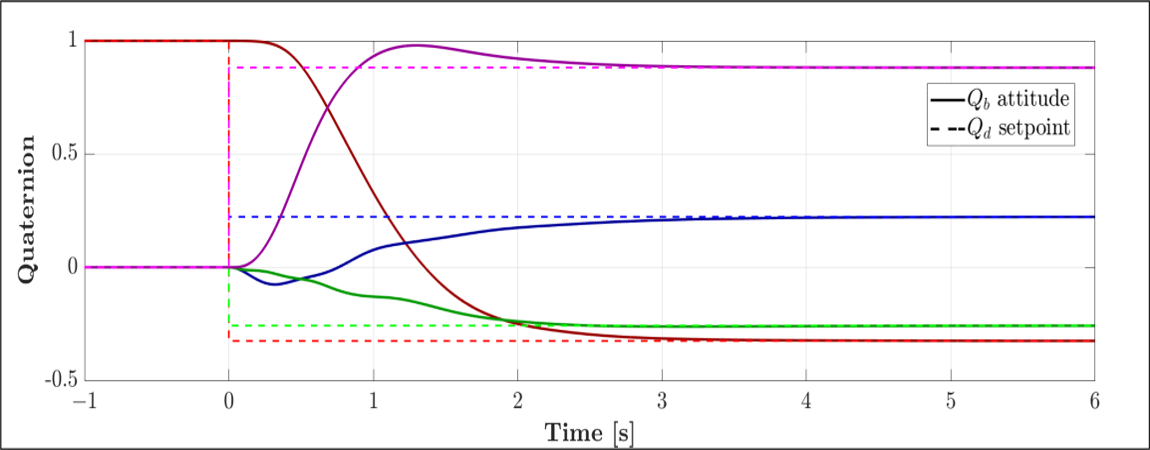
\includegraphics[width=0.45\textwidth]{figs/attitude-step}
\vspace{-8pt}
\caption{Attitude step}
\label{fig:attitude-step}
\end{figure}
\begin{figure}[tbp]
\vspace{-10pt}
\centering
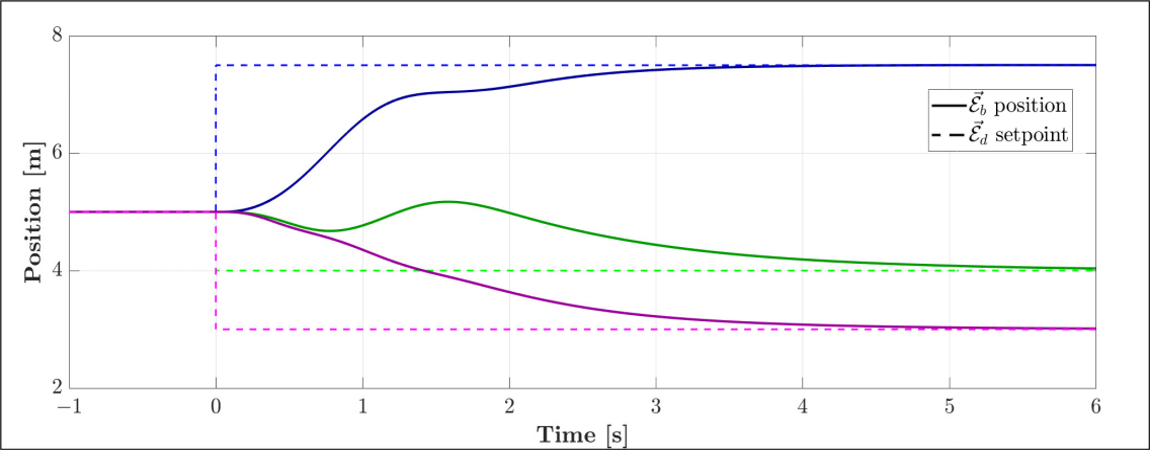
\includegraphics[width=0.45\textwidth]{figs/position-step}
\vspace{-8pt}
\caption{Position step}
\label{fig:position-step}
\vspace{-18pt}
\end{figure}
\par
Step responses for both attitude and position controllers are shown in Fig:\ref{fig:attitude-step}-\ref{fig:position-step} respectively. Neither controllers induced saturation of any actuator for the step and both states settled to 95\% in $t_{95}=5.62~[\text{s}]$. The objective was dynamic setpoint tracking so; to test that, an orbital trajectory was generated and commanded as a state setpoint. The trajectory orbits a central point at $0.5~[\text{Hz}]$, completing one orbit in $120~[\text{s}]$, starting from $Q_b(0)=[1~\vec{0}\hspace{2pt}]^T$ and $\vec{\mathcal{E}}_b(0)=[5~5~5]^T$. Tracking of that trajectory with an oscillating quaternion attitude and inertial position setpoints is shown in Fig:\ref{fig:attitude-trajectory}-\ref{fig:position-trajectory} respectively.
%=========================================================
\section{Conclusion}
\label{sec:conclusion}
%=========================================================
The non-zero setpoint tracking goal for a quadcopter's state is achieved with the control structure(s) proposed. Only first order setpoints were defined in (\ref{eq:angular-error}) and (\ref{eq:velocity-error}) which led to some phase lag in the resultant tracked trajectory. Commanding angular and translational velocity setpoints would diminish such an error. The combination of non-zero attitude and position setpoint tracking is an interesting result for a quadrotor helicopter; the proposed control solutions are expanded and improved upon in \cite{dualaxistilting} wherein exponentially stabilizing control laws are investigated.
\par
\begin{figure}[btp]
\vspace{-12pt}
\centering
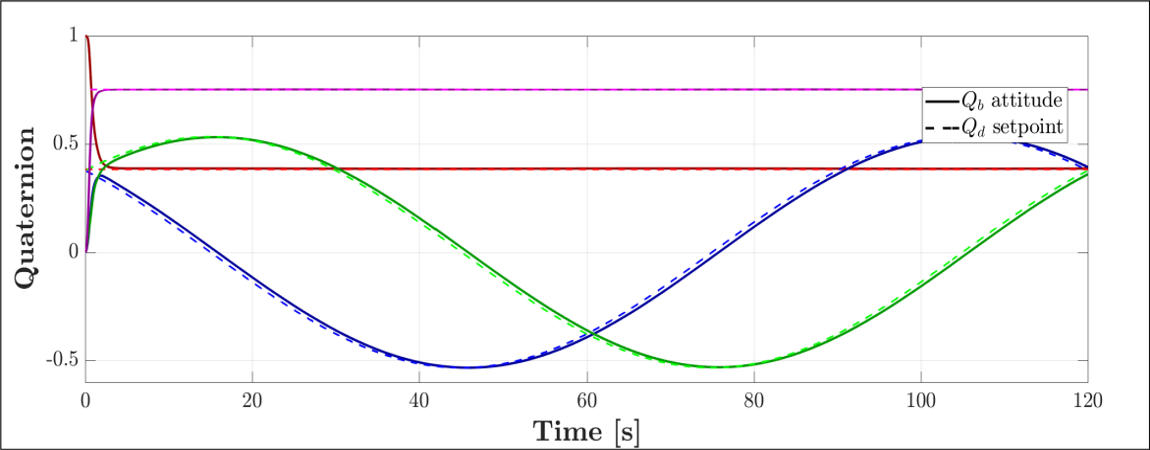
\includegraphics[width=0.45\textwidth]{figs/attitude-trajectory}
\vspace{-8pt}
\caption{Attitude trajectory}
\label{fig:attitude-trajectory}
\end{figure}
\begin{figure}[tbp]
\vspace{-10pt}
\centering
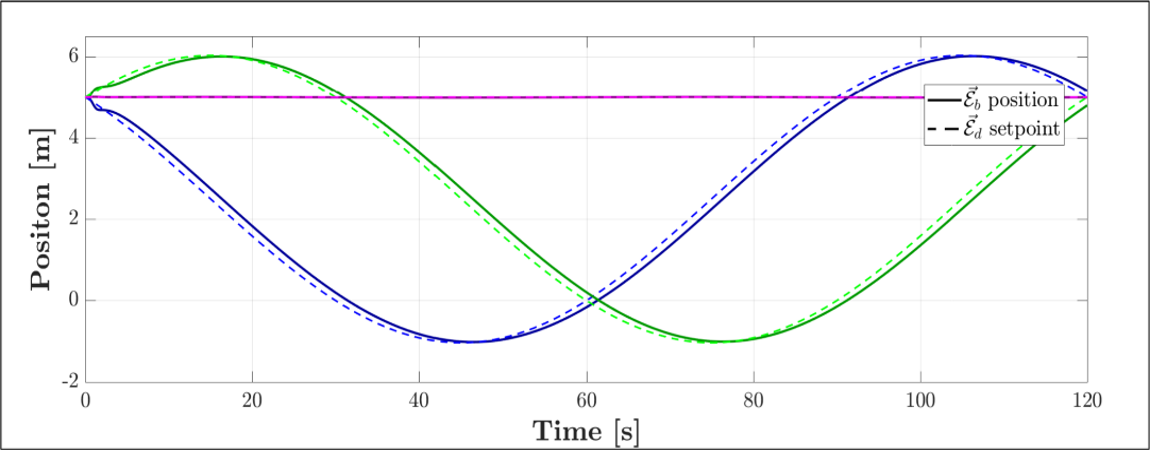
\includegraphics[width=0.45\textwidth]{figs/position-trajectory}
\vspace{-8pt}
\caption{Position trajectory}
\label{fig:position-trajectory}
\end{figure}
\par
The final point of consideration is the application of a pseudo inversion control allocation in (\ref{eq:pseudo-inversion}). Such an inversion, as described in \cite{allocation}, applies a least squares optimization to it's associated actuator matrix. The physical consequence of this is that the magnitude $|\vec{T}_{1\rightarrow 4}|$ for thrust vectors to be commanded is minimized (\emph{optimized}); meaning the control algorithm prioritizes pitching those thrust vectors with $\lambda_i$ or $\alpha_i$ before changing their magnitudes with $\Omega_i$ propeller speed changes\ldots
%=========================================================
\begin{thebibliography}{00}
\bibitem{x4flyer} P. Pounds, R. Mahony, P. Hynes and J. Roberts, "Design of a four-rotor aerial robot",In Friedrich, Werner \& Lim, Patrick, Proceeding of Australasian conference on robotics and automation, pp. 145-150, Nov 2002.
\bibitem{ftcallocation} P. Baldi, B. Mogens, P. Castaldi, N. Mimmo and S. Simani, "Adaptive FTC based on control allocation and fault accommodation for satellite reaction wheels", IEEE, Conference on control and fault-tolerant Systems, vol. 3, pp672--677, Sept 2016.
\bibitem{quaternionbackstep} R. Kristiansen and P.J. Nicklasson, "Satellite attitude control by quaternion-based backstepping", IEEE, Trans. on control systems technology, vol. 17, pp227--232, Jan 2009.
\bibitem{allocation} T.A. Johansen and T.I. Fossen, "Control allocation - a Survey", Automatica, vol. 49, pp1087--1103, Jun 2013.
\bibitem{ggress} G.R. Gress, "Lift fans as gyroscopes for controlling compact VTOL air vehicles: overview and development status of oblique active tilting", American Helicopter Society Forum, vol 63, May 2007.
\bibitem{tiltingmodelling} M. Ryll and H. Bulthoff and P. Robuffo Giordano, "Modelling and control of a quadrotor UAV with tilting propellers", IEEE, Conference on robotics and automation, pp4606--4613, May 2012.
2002.
\bibitem{tiltingtest} M. Ryll and H. Bulthoff and P. Robuffo Giordano, "First flight tests of a quadrotor UAV with tilting propellers", IEEE, Conference on robotics and automation, pp295-302, Dec 2013.
\bibitem{nemati} A. Nemati and M.Kumar, "Modelling and control of a single Axis tilting quadcopter", American control conference, pp3077--3082, Jun 2014.
\bibitem{tiltgasco} P.S. Gasco and Y. Al-Rihani, "Development of a dual-axis tilt rotorcraft UAV", Univ. Cranfield, department of Engineering, Nov 2012.
\bibitem{shoemaker} K. Shoemaker, "Quaternions", Univ. Pennsylvania, Department of computer and information science, 1987.
\bibitem{nonlineardynamics} M. Bangura and R. Mahony, "Non-linear dynamic modeling for high performance control of a quadrotor", Australian robotics and automation association, Conference on robotics and automation, pp1--10, Dec 2012.
\bibitem{lowreynolds} J. Brandt and M. Selig, "Propeller performance data at low Reynolds numbers", American institute of aeronautics and astronatics, Sciences meeting, vol. 49, pp 1--18, Jan 2011.
\bibitem{lagrange} T. Thornton and J.B. Marion, "Classical dynamics of particles and systems", Thompson Brooks/Cole, 5th Edition, Ch 7, pp 228--289, 2003.
\bibitem{bojelyapunov} E. Boje, "Lyapunov stability analysis", Univ. Kwazulu natal, Department of electrical, electronic and eomputer engineering, Control Systems: ENEL4CN, Jan 2005, unpublished.
\bibitem{dualaxistilting} N. Von Klemperer, "Dual-axis tilting quadrotor aircraft", Univ. Cape Town,  Department of Electrical Engineering, Oct 2017, in press.
\bibitem{rotation} D.D. Garanin, "Rotational motion of rigid bodies", Univ. New York, Department of engineering, Nov 2008.
\bibitem{particletrajectories} F. van den Berg, A.P. Engelbrecht, "A study of particle swarm optimization particle trajectories", Univ. Pretoria, Department of computer science, Mar 2005.
\end{thebibliography}
\end{document}
